

\section{PRPs and PRFs}

\begin{definition} [PRP] PRP: 

    Pseudo Random Permutation (PRP) defined over (K,X):
    $\mathrm{E}: \mathrm{K} \times \mathrm{X} \rightarrow \mathrm{X}$
    such that:
    \begin{enumerate} [itemsep=2pt,topsep=0pt,parsep=0pt]
        \item Exists "efficient" deterministic algorithm to evaluate $E(k, x)$
        \item The function $E(k, \cdot)$ is one-to-one
        \item Exists "efficient" inversion algorithm $D(k, y)$
    \end{enumerate}
    
\end{definition}


\begin{definition} [PRF] PRF:

    Pseudo Random Function (PRF) defined over (K,X,Y):
    $F: K \times X \rightarrow Y \rightarrow$ 
    such that exists "efficient" algorithm to evaluate $F(k, x)$

\end{definition}

\subsection{Secure PRFs and Secure PRPs}

From intuition, a PRF is secure if a random function in $Funs[X,Y]$ is indistinguishable from a random function in $S_F$. The experiment for secure PRF is shown in Figure \ref{fig: 03 Secure PRF Experiment}.

\begin{figure}[h]
    \centering
    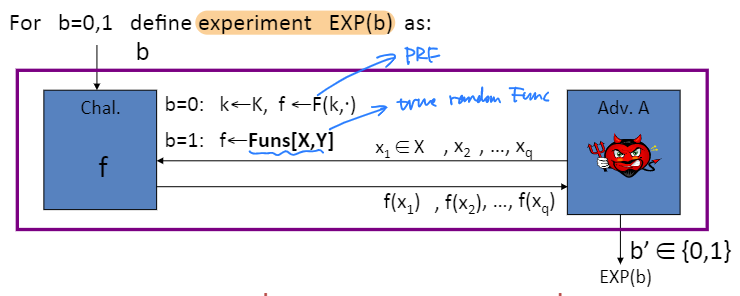
\includegraphics[width=0.5\textwidth]{Stanford_Crypto_1/fig/03_block_cipher/Secure PRF Experiment.png}
    \caption{Secure PRF Experiment}
    \label{fig: 03 Secure PRF Experiment}
\end{figure}

\begin{definition} [Secure PRF] Secure PRF

    $F$ is a secure PRF if for all "efficient" A:
    $$
    \operatorname{Adv}_{\mathrm{PRF}}[A, \mathrm{~F}]:=|\operatorname{Pr}[\operatorname{EXP}(0)=1]-\operatorname{Pr}[\operatorname{EXP}(1)=1]|
    $$
    is "negligible."
    
\end{definition}

The experiment for secure PRF is shown in Figure \ref{fig: 03 Secure PRP Experiment}.

\begin{figure}[h]
    \centering
    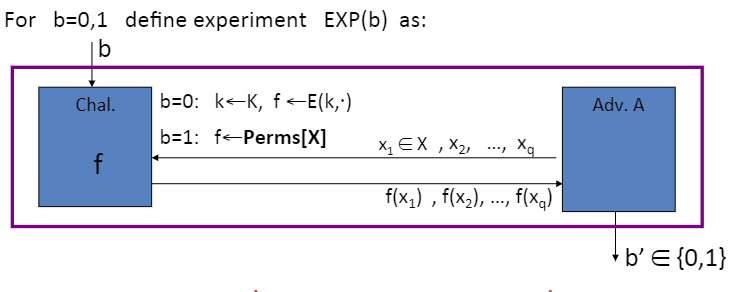
\includegraphics[width=0.5\textwidth]{Stanford_Crypto_1/fig/03_block_cipher/Secure PRP Experiment.png}
    \caption{Secure PRP Experiment}
    \label{fig: 03 Secure PRP Experiment}
\end{figure}

\begin{definition} [Secure PRP] Secure PRP:

    $E$ is a secure PRP if for all "efficient" A:
    $$
    \operatorname{Adv}_{\mathrm{PRP}}[A, E]=|\operatorname{Pr}[\operatorname{EXP}(0)=1]-\operatorname{Pr}[\operatorname{EXP}(1)=1]|
    $$
    is "negligible."
    
\end{definition}

AES, 3DES are PRPs that is believed to be secure.

There is a Lemma about the relation between secure PRP and secure PRF. The lemma tell us that "any secure PRP is also a secure PRF, if $|X|$ is sufficiently large"
 
\begin{lemma} [PRF Switching Lemma] PRF Switching Lemma
    Let $\mathrm{E}$ be a PRP over $(\mathrm{K}, \mathrm{X})$
    Then for any q-query adversary A:
    $$
    \left|\operatorname{Adv}_{\text {PRF }}[A, E]-\operatorname{Adv}_{\text {PRP }}[A, E]\right|<q^{2} / 2|X|
    $$
\end{lemma}


\subsection{Constructing PRGs from PRFs}

\begin{method} [From PRFs to PRGs: 1] From PRFs to PRGs:

    Let $\mathrm{F}: \mathrm{K} \times\{0,1\}^{\mathrm{n}} \rightarrow\{0,1\}^{\mathrm{n}}$ be a secure PRF.
    Then the following $G: K \rightarrow\{0,1\}^{n t} \quad$ is a secure PRG:
    $$
    \mathrm{G}(\mathrm{k})=\mathrm{F}(\mathrm{k}, 0)\|\mathrm{F}(\mathrm{k}, 1)\| \cdots \| \mathrm{F}(\mathrm{k}, \mathrm{t}-1)
    $$
        
\end{method}

One advantage of this method is it is parallelizable.

\subsection{Constructing PRFs from PRGs}

The first method is Tree Construction that helps us generate PRFs from PRGs, the structure of the Tree Construction is shown in Figure \ref{fig: 03 Tree Construction}.

\begin{figure}[h]
    \centering
    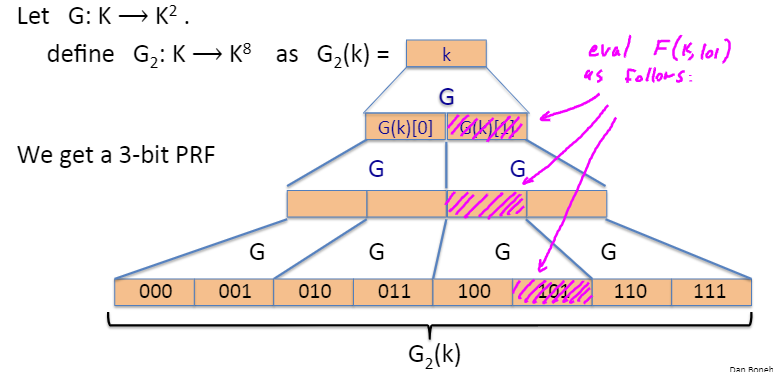
\includegraphics[width=0.5\textwidth]{Stanford_Crypto_1/fig/03_block_cipher/Tree Construction.png}
    \caption{Tree Construction}
    \label{fig: 03 Tree Construction}
\end{figure}

Another method to generate PRFs to PRGs is the GGM PRF method. Which is shown in Figure \ref{fig: 03 GGM PRF}.

\begin{figure}[h]
    \centering
    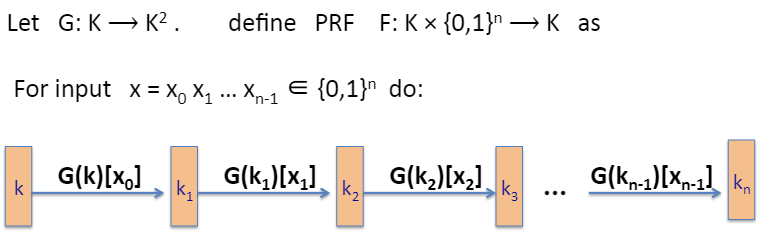
\includegraphics[width=0.5\textwidth]{Stanford_Crypto_1/fig/03_block_cipher/GGM PRF.png}
    \caption{GGM PRF}
    \label{fig: 03 GGM PRF}
\end{figure}

However, this method is quite slow, so it is not used in practice.

A property exists for these two methods: \textbf{If G is a secure PRG then the F is a secure PRF}


\section{Block Ciphers}

The structure of the block cipher is shown in Figure \ref{fig: 03 Block Cipher}.

\begin{figure}[h]
    \centering
    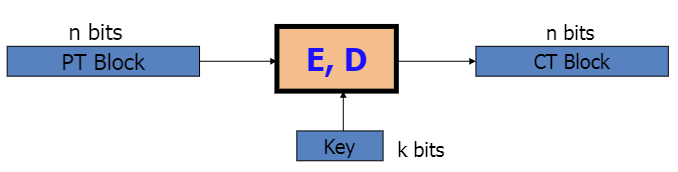
\includegraphics[width=0.8\textwidth]{Stanford_Crypto_1/fig/03_block_cipher/Block Cipher.png}
    \caption{Block Cipher}
    \label{fig: 03 Block Cipher}
\end{figure}

The general framework of the block cipher is shown in Figure \ref{fig: 03 Block Cipher Structure}

\begin{figure}[h]
    \centering
    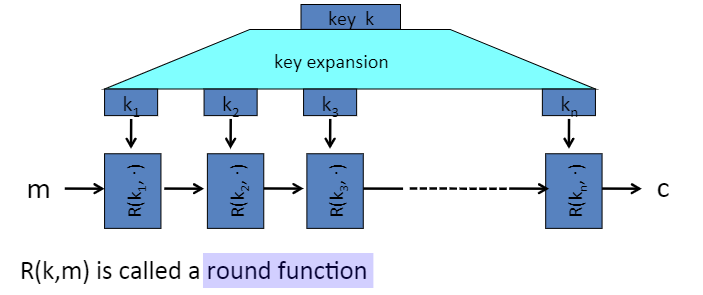
\includegraphics[width=0.8\textwidth]{Stanford_Crypto_1/fig/03_block_cipher/Block Cipher Structure.png}
    \caption{Block Cipher Structure}
    \label{fig: 03 Block Cipher Structure}
\end{figure}

\subsection{The Data Encryption Standard (DES)}

    The DES encryption algorithm is a \textbf{16-round Feistel network} where each round uses a different function $f: \mathcal{X} \rightarrow \mathcal{X}$(round function).

\subsubsection{Feistel Network}

The encryption process of Feistel Network is shown in Figure \ref{fig: 03 Feistel Network Encryption}.

\begin{figure}[h]
    \centering
    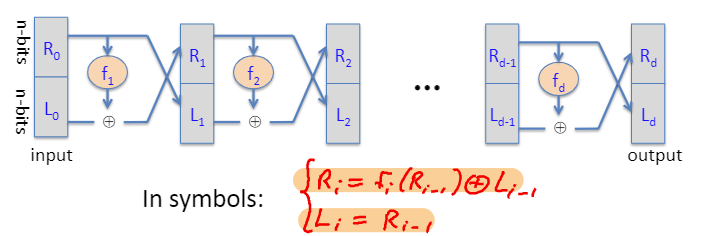
\includegraphics[width=0.8\textwidth]{Stanford_Crypto_1/fig/03_block_cipher/Feistel Network Encryption.png}
    \caption{Feistel Network Encryption}
    \label{fig: 03 Feistel Network Encryption}
\end{figure}


The decryption process of Feistel Network is shown in Figure \ref{fig: 03 Feistel Network Decryption}.

\begin{figure}[h]
    \centering
    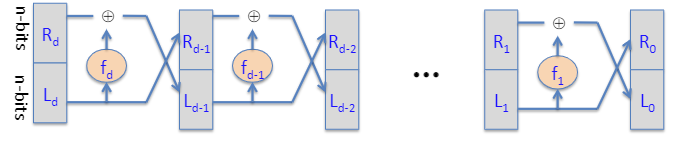
\includegraphics[width=0.8\textwidth]{Stanford_Crypto_1/fig/03_block_cipher/Feistel Network Decryption.png}
    \caption{Feistel Network Decryption}
    \label{fig: 03 Feistel Network Decryption}
\end{figure}

The inversion part is basically the same circuit with $f_1 , \cdots f_d$ applied in reverse order.

\begin{theorem} [Theorem about Security of Feistel Network] Theorem about Security of Feistel Network:

    f: $\mathrm{K} \times\{0,1\}^{\mathrm{n}} \rightarrow\{0,1\}^{\mathrm{n}}$ a secure PRF
    $\Rightarrow$ 3-round Feistel $\mathrm{F}: \mathrm{K}^{3} \times\{0,1\}^{2 \mathrm{n}} \rightarrow\{0,1\}^{2 \mathrm{n}}$ a secure PRP
    
\end{theorem}

\subsection{DES Round Function}

In round number $i$ the function $f$ is defined as
$$
f(x):=F\left(k_{i}, x\right)
$$
where $k_{i}$ is a 48 -bit key for round number $i$ and $F$ is a fixed function called the DES round function. The function $F$ is the centerpiece of the DES algorithm and is shown in Figure \ref{fig: 03 DES Round Function}.

\begin{figure}[h]
    \centering
    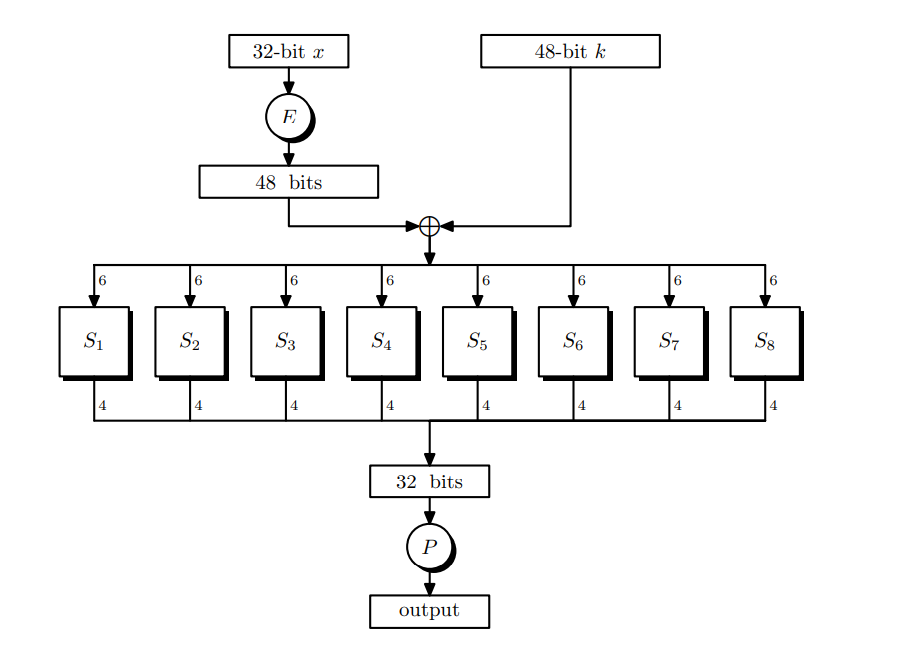
\includegraphics[width=0.8\textwidth]{Stanford_Crypto_1/fig/03_block_cipher/DES Round Function.png}
    \caption{DES Round Function}
    \label{fig: 03 DES Round Function}
\end{figure}

The auxiliary functions in the round function is shown as follows

\begin{enumerate} [itemsep=2pt,topsep=0pt,parsep=0pt]
    \item The function $E$ expands a 32-bit input to a 48-bit output by rearranging and replicating the input bits. For example, $E$ maps input bit number 1 to output bits 2 and 48 ; it maps input bit 2 to output bit number 3 , and so on.
    \item The function $P$, called the mixing permutation, maps a 32 -bit input to a 32 -bit output by rearranging the bits of the input. For example, $P$ maps input bit number 1 to output bit number 9 ; input bit number 2 to output number 15 , and so on.
    \item At the heart of the DES algorithm are the functions $S_{1}, \ldots, S_{8}$ called S-boxes. Each S-box $S_{i}$ maps a 6-bit input to a 4-bit output by a lookup table. The DES standard lists these 8 look-up tables, where each table contains 64 entries.
\end{enumerate}

It is important to choose appropriate S-BOXES and P-BOXES.

\subsubsection{Triple DES}

For Normal DES with a 56-bit cipher, it can be broken in 7 days. So we need more method to make DES more safety under exhausitve search attack.

\begin{method} [Triple DES]

    The Triple-DES standard. NIST approved Triple-DES for government use through the ycar 2030. Strictly speaking, the NIST version of Triplc-DES is defined as
    $$
    E_{3}\left(\left(k_{1}, k_{2}, k_{3}\right), x\right):=E\left(k_{3}, D\left(k_{2}, E\left(k_{1}, x\right)\right)\right) .
    $$
    
\end{method}

The reason for this is that setting $k_{1}=k_{2}=k_{3}$ reduces the NIST Triple-DES to ordinary DES and hence Triple-DES hardware can be used to implement single DES.

\subsubsection{Meet in the Middle Attack}

The problem is why we do not use a Double-DES. The problem is for Double-DES there is an efficient attack: Meet in the Middle Attack. The structure of meet in the middle attack is shown in Figure \ref{fig: 03 DES Meet in the Middle Attack}.

\begin{figure}[h]
    \centering
    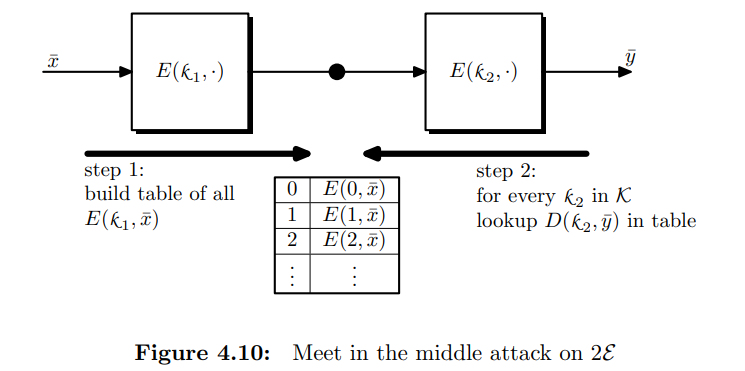
\includegraphics[width=0.8\textwidth]{Stanford_Crypto_1/fig/03_block_cipher/DES Meet in the Middle Attack.png}
    \caption{DES Meet in the Middle Attack}
    \label{fig: 03 DES Meet in the Middle Attack}
\end{figure}

\subsubsection{DESX}

Another method is DESX.

\begin{method} [DESX] DESX: 

    \begin{equation}
        \begin{aligned}
            &\mathrm{E}: \mathrm{K} \times\{0,1\}^{\mathrm{n}} \longrightarrow\{0,1\}^{\mathrm{n}} \text { a block cipher } \\
            &\text { Define } E X \text { as } \operatorname{EX}\left(\left(\mathrm{k}_{1}, \mathrm{k}_{2}, \mathrm{k}_{3}\right), \mathrm{m}\right)=\mathrm{k}_{1} \oplus \mathrm{E}\left(\mathrm{k}_{2}, \mathrm{~m} \oplus \mathrm{k}_{3}\right) \\
            &\text { For DESX: } \text { key-len }=64+56+64=184 \text { bits } \\
        \end{aligned}
    \end{equation}
    
\end{method}

DESX has an easy attack in time $2^{64+56}=2^{120}$ compared to its key length


\subsection{AES}

The high level overview of AES is shown in Figure \ref{fig: 03 AES High-level}. It is a substitution-permutation network.

\begin{figure}[h]
    \centering
    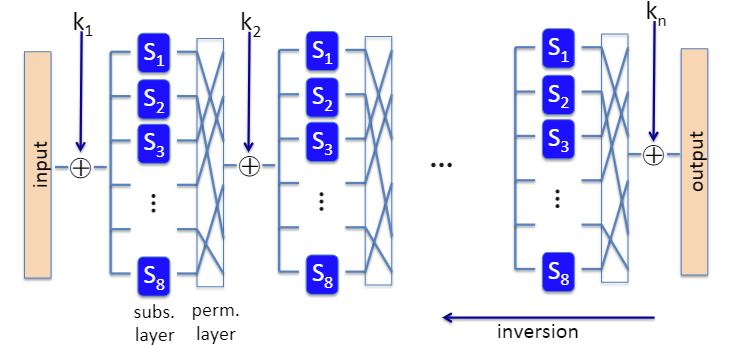
\includegraphics[width=0.8\textwidth]{Stanford_Crypto_1/fig/03_block_cipher/AES High-level.png}
    \caption{AES High-level}
    \label{fig: 03 AES High-level}
\end{figure}


\subsubsection{Schematic of AES-128}

The schematic of AES-128 is shown in Figure \ref{fig: 03 AES128 Schematic}.

\begin{figure}[h]
    \centering
    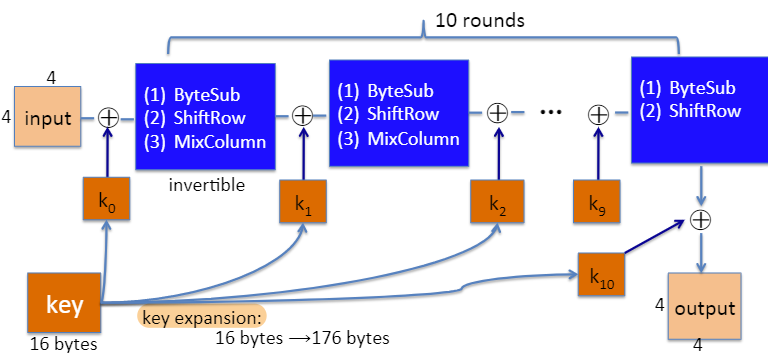
\includegraphics[width=0.8\textwidth]{Stanford_Crypto_1/fig/03_block_cipher/AES128 Schematic.png}
    \caption{AES128 Schematic}
    \label{fig: 03 AES128 Schematic}
\end{figure}

The auxiliary functions of AES is shown as follows:

\begin{enumerate}
    \item ByteSub: $A[i, 7]) \in S[A(i, J)]$
    \item ShiftRows: shown in Figure \ref{fig: 03 AES Auxialiary Functions}.
    \item MixColumns: shown in Fiugre \ref{fig: 03 AES Auxialiary Functions}
\end{enumerate}

\begin{figure}[h]
    \subfigure[ShiftRows]{
        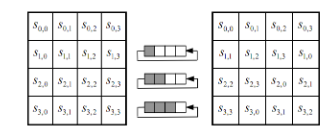
\includegraphics[width=0.5\textwidth]{Stanford_Crypto_1/fig/03_block_cipher/AES Shift Rows.png}
    }
    \subfigure[Mix Columns]{
        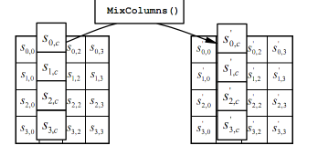
\includegraphics[width=0.5\textwidth]{Stanford_Crypto_1/fig/03_block_cipher/AES Mix Columns.png}
    }
    \caption{AES Auxialiary Functions}
    \label{fig: 03 AES Auxialiary Functions}
    
\end{figure}


\section{Security of Block Ciphers}

\subsection{Exhaustive Search Attacks}

The goal of exhaustive search attack is: given a few input output pairs $(m_i,c_i=E(k,m_i))$, find key.


\subsection{Semantic Security for Many-Time Key}

For the many-time key cases, the adversary is able to see many CTs with same key.

\begin{definition} [Chosen-Plaintext Attack(CPA)] Chosen-Plaintext Attack(CPA)

    The adversary is able to obtain the encryption of arbitrary messages of his choice.
    
\end{definition}

The attack game of many-time key is shown in Figure \ref{fig: 03 Attack of Sem Secure for Many-Time Key}.

\begin{figure}[h]
    \centering
    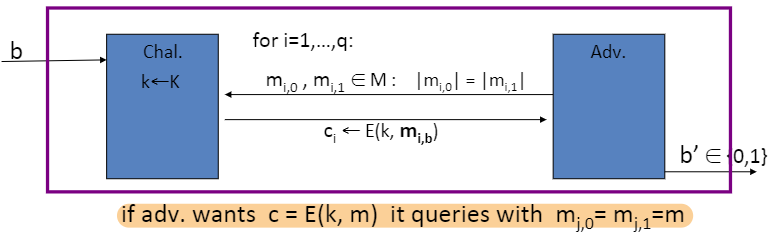
\includegraphics[width=0.8\textwidth]{Stanford_Crypto_1/fig/03_block_cipher/Attack of Sem Secure for Many-Time Key.png}
    \caption{Attack of Sem Secure for Many-Time Key}
    \label{fig: 03 Attack of Sem Secure for Many-Time Key}
\end{figure}

\begin{definition} [Sem. Sec with CPA]

    E is sem. sec. under CPA if for all "efficient" A:
    $$
    \operatorname{Adv}_{\text {CPA }}[A, E]=|\operatorname{Pr}[\operatorname{EXP}(0)=1]-\operatorname{Pr}[\operatorname{EXP}(1)=1]|
    $$
    is "negligible."
    
\end{definition}

If a system is not Sem. Sec. with CPA, this means an attacker can learn that two encrypted files are the same or two encrypted packets are the same. This is malicious, because like in a voice stream, the attacker will know the break time.

\subsubsection{Property}

Suppose $E(k,m)$ always outputs the same ciphertext for msg m, then it will not be secure with CPA (shown in Figure \ref{fig: 03 Ciphers Insecure under CPA}).

\begin{figure}[h]
    \centering
    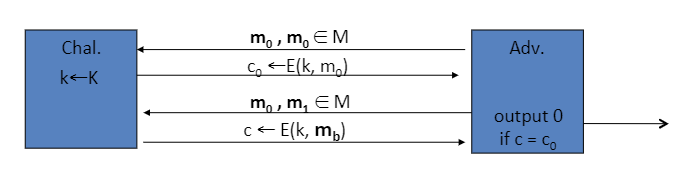
\includegraphics[width=0.8\textwidth]{Stanford_Crypto_1/fig/03_block_cipher/Ciphers Insecure under CPA.png}
    \caption{Ciphers Insecure under CPA}
    \label{fig: 03 Ciphers Insecure under CPA}
\end{figure}

This means, if a secret key is to be used multiple times, we should have: given the same plaintext message twice, the encryption must produce different outputs.

\subsubsection{Solution 1: Randomized Encryption}

The structure of the randomized encryption is shown in Figure \ref{fig: 03 Randomized Encrpytion}.

\begin{figure}[h]
    \centering
    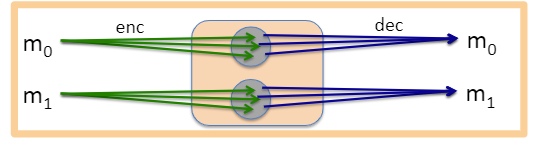
\includegraphics[width=0.8\textwidth]{Stanford_Crypto_1/fig/03_block_cipher/Randomized Encrpytion.png}
    \caption{Randomized Encryption}
    \label{fig: 03 Randomized Encrpytion}
\end{figure}

Which means we should use a $E(k,m)$ that is a randomized algorithm. However, it also means the ciphertext must be longer than plaintext. (because it is a one to n mapping)

\subsubsection{Solution 2: Nonce-Based Encryption}

\begin{definition} [nonce] nonce

    a value that changes from msg to msg.

    (k,n) pair never used more than once
    
\end{definition}

The structure of the nonce-based encryption is shown in Figure \ref{fig: 03 Nonce-Based Encryption}.


\begin{figure}[h]
    \centering
    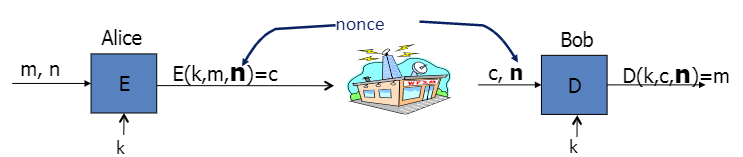
\includegraphics[width=0.8\textwidth]{Stanford_Crypto_1/fig/03_block_cipher/nonce-based encrpytion.png}
    \caption{Nonce-Based Encryption}
    \label{fig: 03 Nonce-Based Encryption}
\end{figure}

There are mainly two ways to define a nonce:
\begin{itemize} [itemsep=2pt,topsep=0pt,parsep=0pt]
    \item nonce is a counter, this is used when encryptor keeps state from msg to msg
    \item encryptor chooses a random nonce
\end{itemize}

The attack of nonce-based encryption is shown in Figure \ref{fig: 03 Attack for nonce-based encryption}.

\begin{figure}[h]
    \centering
    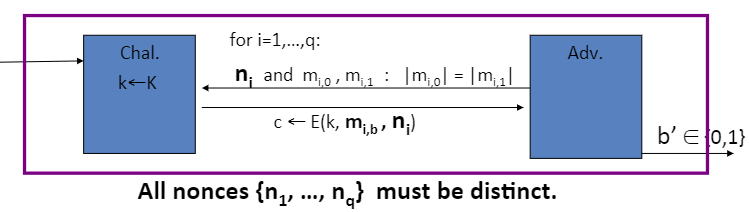
\includegraphics[width=0.8\textwidth]{Stanford_Crypto_1/fig/03_block_cipher/Attack for nonce-based encryption.png}
    \caption{Attack for nonce-based encryption}
    \label{fig: 03 Attack for nonce-based encryption}
\end{figure}

\begin{definition} [Sem.Secure for Nonce-Based E under CPA] Sem.Secure for Nonce-Based E under CPA:

    nonce-based $E$ is sem. sec. under CPA if for all "efficient" A:
    $\operatorname{Adv}_{\text {nCPA }}[A, E]=|\operatorname{Pr}[\operatorname{EXP}(0)=1]-\operatorname{Pr}[\operatorname{EXP}(1)=1]|$ is "negligible."
    
\end{definition}


\subsection{More Attacks on Block Ciphers}


\subsubsection{Attacks on the implementation}

There  are a lot of method to attack block cipher based on the implementation. So the main lesson is: \textbf{Don't Design Ciphers Yourself}



\subsection{Modes of Operations}

\subsection{ECB: An Incorrect Use of a PRP}


The electronic Code Block is a classical incorrect way of using a PRP. The structure of ECB is shown in Figure \ref{fig: 03 ECB Mode}.


\begin{figure}[h]
    \centering
    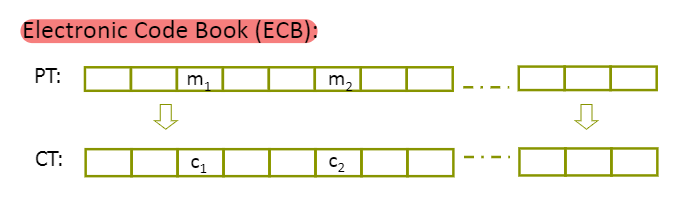
\includegraphics[width=0.8\textwidth]{Stanford_Crypto_1/fig/03_block_cipher/ECB Mode.png}
    \caption{ECB Mode}
    \label{fig: 03 ECB Mode}
\end{figure}


The problem of ECB is for the same message $m_1=m_2$ it will produce the same ciphertext $c_1=c_2$. So it will lost the CPA Attack.



\subsection{CBC with random IV}

CBC: Cipher Block Chain

IV: Initial Vector

The encrpytion and decryption process of CBC with random IV is shown in Figure \ref{fig: 03 CBC with random IV}.

\begin{figure}[h]
    \subfigure[Encryption]{
        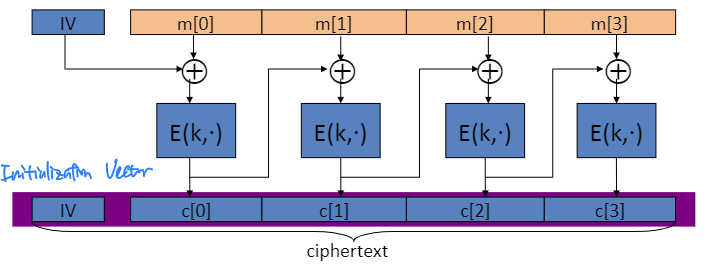
\includegraphics[width=0.5\textwidth]{Stanford_Crypto_1/fig/03_block_cipher/CBC with Random IV Encry.png}
    }
    \subfigure[Decyprtion]{
        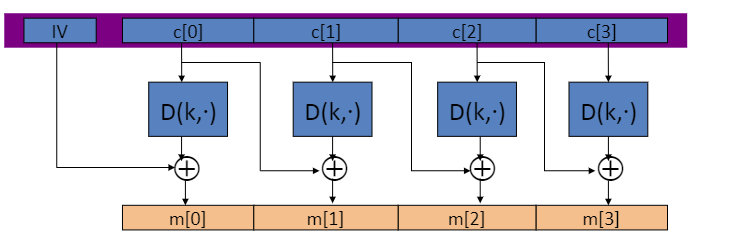
\includegraphics[width=0.5\textwidth]{Stanford_Crypto_1/fig/03_block_cipher/CBC with Random IV Decry.png}
    }
    \caption{CBC with random IV}
    \label{fig: 03 CBC with random IV}
\end{figure}

\subsubsection{Nonce-Based CBC}

The nonce-based CBC use a key pair $key=(k,k_1)$. It is a CBC with unique nonce, i.e. (key,n) pair is used for only one message. The structure of the nonce-based CBC is shown in Figure \ref{fig: 03 nonce-based CBC}.

\begin{figure}[h]
    \centering
    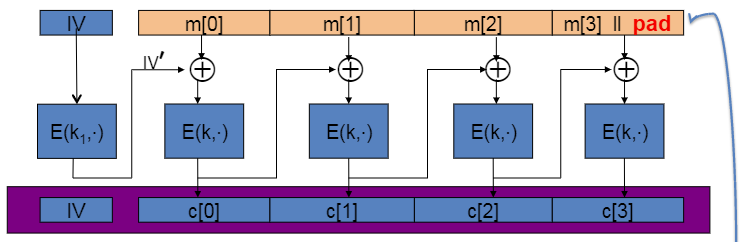
\includegraphics[width=0.8\textwidth]{Stanford_Crypto_1/fig/03_block_cipher/nonc-based CBC.png}
    \caption{Nonce-based CBC}
    \label{fig: 03 nonce-based CBC}
\end{figure}

\subsubsection{Padding in CBC}

The CBC mode need a padding part to extend the message in order to let the length becomes a multiple of block size. The pad is removed during decryption.

One example is the padding used in the TLS: for $n>0, n$ byte pad is \begin{tabular}{|l|l|l|l|l|} \hline$n$ & $n$ & $n$ & $\cdots$ & $n$ \\ \hline \end{tabular}
if no pad needed, add a dummy block


\subsubsection{CPA Security}

\begin{theorem} [CBC CPA Security]
    For any $L>0$,
    If $E$ is a secure PRP over $(K, X)$ then
    $E_{C B C}$ is a sem. sec. under $C P A$ over $\left(K, X^{L}, X^{L+1}\right)$.
    In particular, for a q-query adversary $A$ attacking $E_{C B C}$ there exists a PRP adversary B s.t.:
    $\operatorname{Adv}_{\mathrm{CPA}}\left[A, E_{\mathrm{CBC}}\right] \leq 2 \cdot \operatorname{Adv}_{\mathrm{PRP}}[B, E]+2 q^{2} L^{2} /|X|$
\end{theorem}

Based on the theorem, we know that after $w^{48}$ AES blocks, we must change key.

\textbf{Notes: } CBC where attacker can predict the IV is not CPA-secure.



\subsection{Random Counter(ctr) Mode}

Let $\mathrm{F}: \mathrm{K} \times\{0,1\}^{\mathrm{n}} \rightarrow\{0,1\}^{\mathrm{n}}$ be a secure PRF.
$\mathrm{E}(\mathrm{k}, \mathrm{m}):$ choose a random $\mathrm{IV} \in\{0,1\}^{\mathrm{n}}$.

Then the structure of the rand ctr-mode is shown in the Figure \ref{fig: 03 rand ctr-mode}.

\begin{figure}[h]
    \centering
    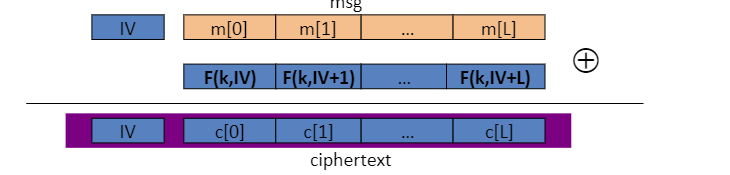
\includegraphics[width=0.8\textwidth]{Stanford_Crypto_1/fig/03_block_cipher/rand ctr-mode.png}
    \caption{rand ctr-mode}
    \label{fig: 03 rand ctr-mode}
\end{figure}

This is a \textbf{parallelizable structure}

\subsubsection{Nonce-Based ctr mode}


\subsubsection{CPA Security}

\begin{theorem} [CPA Security for CTR Mode] CPA Security for CTR Mode:

    Counter-mode Theorem: For any $L>0$,
    If $F$ is a secure PRF over $(K, X, X)$ then
    $E_{C T R}$ is a sem. sec. under CPA over $\left(K, X^{L}, X^{L+1}\right)$.
    In particular, for a q-query adversary $A$ attacking $E_{C T R}$
    there exists a PRF adversary B s.t.:
    $\operatorname{Adv}_{\mathrm{CPA}}\left[A, E_{\mathrm{CTR}}\right] \leq 2 \cdot \operatorname{Adv}_{\mathrm{PRF}}[B, F]+2 q^{2} L /|X|$
    
\end{theorem}

ctr-mode only secure as long as $q^{2} L<|X|$. Better than $C B C$. Based on the theorem, if we use AES in CTR mode, after $2^32$ CTs each of len $2^32$, we must change key. 

\section{Summary}
This chapter, we start from PRP and PRF. We defined what is secure PRF and secure PRP. And we propose method to construct PRF or PRG from each other. 

Then we introduce two useful method of block cipher: AES and DES. AES is much more safer while DES is less safer and we always use 3-DES.

Then we define the model of CPA Sem. Sec. Based on the CPA Sem. Sec., we knows that if we want to use the same key many times and keep safe, we need to let the same message generate different ciphertext. Based on that, we need the randomized algorithm or nonce-based algorithm. Which means we need to use PRG or PRF.

Besides, although we use some randomized component, how to use it is also a big problem. We knows that ECB is not secure. Classical secure modes of operation contains: CBC mode and CTR mode.